\newpage
\section{Quantum Algorithms}

\subsection{Reversibility and Quantum Parallelism}

\subsubsection{The General Computational Process}
A computation is a map
\begin{align*}
    f: x\leftarrow f(x)
\end{align*}
where $x$ is an $n$-bit integer, and $f(x)$ is an m-bi integer. The total resources are at least, $n+m$ qubits. 

In a quantum computer, the computation is achieved by applying a unitary transformation $U_f$ to the $n+m$ qubits. 
\begin{align*}
    U_f(\ket{x}_n\ket{y}_m)=\ket{x}_n\ket{y\oplus f(x)}_m
\end{align*}
where $\oplus$ represents the bitwise exclusive OR, or mod-2 addition. For example,
\begin{align*}
    110010\oplus 010101=100111
\end{align*}

\subsubsection{Reversibility}
The computation is reversible
\begin{align*}
    U_f U_f (\ket{x}_n\ket{y}_m)&=U_f (\ket{x}_n\ket{y\oplus f(x)}_m)\\
    &=\ket{x}_n | y\oplus \underbrace{f(x) \oplus f(x)}_{\forall z,\ z\oplus z=0} \rangle_m\\
    &=\ket{x}_n\ket{y}_m 
\end{align*}

In particular, when $y=0$,
\begin{align*}
    U_f(\ket{x}_n\ket{0}_m)=\ket{x}_n\ket{f(x)}_m
\end{align*}

\subsubsection{Quantum Parallelism}
Let us illustrate why, in principle, a quantum computer can achieve superior performance to their classical counterpart.

\begin{align*}
    H\ket{0}&=\frac{1}{\sqrt{2}}(\ket{0}+\ket{1})\\
    H\otimes H(\ket{0}\otimes \ket{0})&=(H\ket{0})\otimes(H\ket{0})\\
    &=\frac{1}{\sqrt{2}}(\ket{0}+\ket{1})\otimes\frac{1}{\sqrt{2}}(\ket{0}+\ket{1})\\
    &=\frac{1}{2}(\ket{00}+\ket{01}+\ket{10}+\ket{11})
\end{align*}

In general, 
\begin{align*}
    H^{\otimes n}\ket{0}_n=\frac{1}{2^{n/2}}\sum_{0\le x<2^n}\ket{x}_n
\end{align*}
where $H^{\otimes n}=\underbrace{H\otimes H\otimes \cdots \otimes H}_{n\text{ times}}$.

Therefore, we seems to calculate in parallel universes.
\begin{align*}
    U_f(H^{\otimes n}\otimes I_m)(\ket{0}_n\ket{0}_m)&=\frac{1}{2^{n/2}}\sum_{0\le x <2^n}U_f(\ket{x}_n\ket{0}_m)\\
    &=\frac{1}{2^{n/2}}\sum_{0\le x <2^n}\ket{x}_n\ket{f(x)}_m
\end{align*}

The quantum advantage is that the (unknown) state encodes the possibilities of extracting the information of $f(x )$ for all $x$ . But how do we find out what the state is? 

Fortunately, it is sufficient to show that a quantum computer can perform tricks, though in very limited cases, that no classical computer can accomplish. As examples, we will cover
\begin{enumerate}\small
    \item Deutsch's algorithm
    \item Grover's search algorithm
\end{enumerate}

\subsection{Deutsch's Trick}
\subsubsection{The Deutsch Problem}
There exist only four different 1-qubit functions:
\begin{figure}[H]
    \centering
    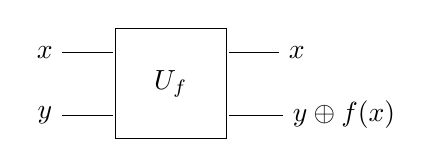
\begin{tikzpicture}
        \node (U) at (0,0) [rectangle, draw=black, minimum height=4em, minimum width=4em, text centered] {$U_f$};

        \node (x) at (-1.6, 0.4) {$\ket{x}$};
        \node (y) at (-1.6, -0.4) {$\ket{y}$};
        
        \draw (x)--(-0.74, 0.4);
        \draw (y)--(-0.74, -0.4);

        \node (x) at (1.6, 0.4) {$\ket{x}$};
        \node (y) at (2.2, -0.4) {$\ket{y\oplus f(x)}$};
        
        \draw (x)--(0.74, 0.4);
        \draw (y)--(0.74, -0.4);
    \end{tikzpicture}
\end{figure}

The four functions are $0,\ x,\ \bar{x},\ 1$. Or explicitly, notice that, with the truth table or the Venn diagram, one can prove
\begin{align*}
    A\oplus B=\overline{A}\oplus \overline{B}
\end{align*}

\begin{enumerate}
    \item $U_f =I_4 $:
    \subitem $\ f_1(0)=f_1(1)=0$
    \begin{figure}[H]
        \centering
        \begin{tikzpicture}
            \node (x) at (-1.6, 0.4) {$\ket{x}$};
            \node (y) at (-1.6, -0.4) {$\ket{y}$};
    
            \node (xx) at (1.6, 0.4) {$\ket{x}$};
            \node (yy) at (1.9, -0.4) {$\ket{y\oplus 0}$};
            
            \draw (x)--(xx);
            \draw (y)--(yy);
        \end{tikzpicture}
    \end{figure}
    
    \item $U_f =CNOT $:
    \subitem $\ f_2(0)=0,\ f_2(1)=1$
    \begin{figure}[H]
        \centering
        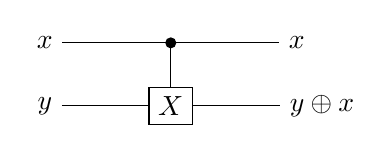
\begin{tikzpicture}
            \node (x) at (-1.6, 0.4) {$\ket{x}$};
            \node (y) at (-1.6, -0.4) {$\ket{y}$};
    
            \node (xx) at (1.6, 0.4) {$\ket{x}$};
            \node (yy) at (1.92, -0.4) {$\ket{y\oplus x}$};

            \node (X) at (0, -0.4) [rectangle, draw=black] {$X$};

            \fill (0, 0.4) circle (2pt);
            
            \draw (x)--(xx);
            \draw (y)--(X);
            \draw (X)--(yy);
            \draw (X)--(0, 0.4);
        \end{tikzpicture}
    \end{figure}
    \item $U_f =CNOT(I_2\otimes X) $:
    \subitem $\ f_3(0)=1,\ f_3(1)=0$
    \begin{figure}[H]
        \centering
        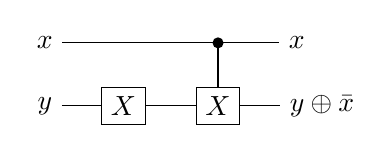
\begin{tikzpicture}
            \node (x) at (-1.6, 0.4) {$\ket{x}$};
            \node (y) at (-1.6, -0.4) {$\ket{y}$};
    
            \node (xx) at (1.6, 0.4) {$\ket{x}$};
            \node (yy) at (1.92, -0.4) {$\ket{y\oplus \bar{x}}$};

            \node (X) at (0.6, -0.4) [rectangle, draw=black] {$X$};
            \node (XX) at (-0.6, -0.4) [rectangle, draw=black] {$X$};

            \fill (0.6, 0.4) circle (2pt);
            
            \draw (x)--(xx);
            \draw (y)--(XX);
            \draw (XX)--(X);
            \draw (X)--(yy);
            \draw (X)--(0.6, 0.4);
        \end{tikzpicture}
    \end{figure}
    \item $U_f =(I_2 \otimes X) $:
    \subitem $\ f_4(0)=f_1(1)=1$
    \begin{figure}[H]
        \centering
        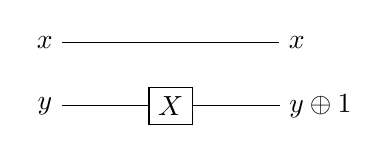
\begin{tikzpicture}
            \node (x) at (-1.6, 0.4) {$\ket{x}$};
            \node (y) at (-1.6, -0.4) {$\ket{y}$};
    
            \node (xx) at (1.6, 0.4) {$\ket{x}$};
            \node (yy) at (1.9, -0.4) {$\ket{y\oplus 1}$};

            \node (X) at (0, -0.4) [rectangle, draw=black] {$X$};

            % \fill (0, 0.4) circle (2pt);
            
            \draw (x)--(xx);
            \draw (y)--(X);
            \draw (X)--(yy);
            % \draw (X)--(0, 0.4);
        \end{tikzpicture}
    \end{figure}
\end{enumerate}

Suppose that we are given a blackbox that executes $U_f$ for one of the four functions. What can we learn about $f$, if we let the box act once?

Remarkably, with a quantum computer we do not have to run $U_f$ twice to determine whether or not $f$ is a constant.

\subsubsection{An Intuitive Trial}
The standard trick, as we discussed on quantum parallelism, is to put the input qubit into the equal superposition of $\ket{0}$ and $\ket{1}$ before the application of $U_f$.

\begin{figure}[H]
    \centering
    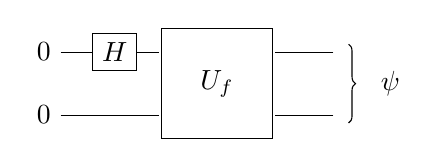
\begin{tikzpicture}
        \node (U) at (0,0) [rectangle, draw=black, minimum height=4em, minimum width=4em, text centered] {$U_f$};

        \node (x) at (-2.2, 0.4) {$\ket{0}$};
        \node (y) at (-2.2, -0.4) {$\ket{0}$};
        \node (H) at (-1.3, 0.4) [rectangle, draw=black] {$H$};
        

        \draw (x)--(H);
        \draw (H)--(-0.74, 0.4);
        \draw (y)--(-0.74, -0.4);

        \node (x) at (1.6, 0.4) { };
        \node (y) at (1.6, -0.4) { };
        
        \draw (x)--(0.74, 0.4);
        \draw (y)--(0.74, -0.4);
        \draw[decorate,decoration={brace,raise=2pt}] (1.6, 0.5)--(1.6, -0.5);

        \node at (2.2, 0) {$\ket{\psi}$};
    \end{tikzpicture}
\end{figure}

We obtain
\begin{align*}
    \ket{\psi}=\frac{1}{\sqrt{2}}(\ket{0}\ket{f(0)}+\ket{1}\ket{f(1)})
\end{align*}

By applying Hadamards to both qubits we obtain
\begin{align*}
    f_1(0)=f_1(1)=0,\ &H\otimes H\ket{\psi}=\frac{1}{\sqrt{2}}\ket{0}(\ket{0}+\ket{1})\\
    f_2(0)=0,\ f_2(1)=1,\ &H\otimes H\ket{\psi}=\frac{1}{\sqrt{2}}(\ket{00}+\ket{11})\\
    f_3(0)=1,\ f_3(1)=0,\ &H\otimes H\ket{\psi}=\frac{1}{\sqrt{2}}(\ket{00}-\ket{11})\\
    f_4(0)=f_4(1)=1,\ &H\otimes H\ket{\psi}=\frac{1}{\sqrt{2}}\ket{0}(\ket{0}-\ket{1})
\end{align*}

Now measure both qubits. Half the time we obtain 00 and know nothing. Half the time, we either get 01, so $f (0) = f (1)$, or 11, so $f (0) \ne f (1)$. We have a 50\% chance of success; one cannot do any better by replacing $H \otimes H$ by other operators.

\subsubsection{The Deutsch Algorithm}
A 100\%-effective method is the following.

\begin{figure}[H]
    \centering
    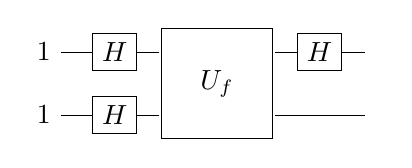
\begin{tikzpicture}
        \node (U) at (0,0) [rectangle, draw=black, minimum height=4em, minimum width=4em, text centered] {$U_f$};

        \node (x) at (-2.2, 0.4) {$\ket{1}$};
        \node (y) at (-2.2, -0.4) {$\ket{1}$};
        \node (H) at (-1.3, 0.4) [rectangle, draw=black] {$H$};
        \node (HH) at (-1.3, -0.4) [rectangle, draw=black] {$H$};
        

        \draw (x)--(H);
        \draw (H)--(-0.74, 0.4);
        \draw (y)--(HH);
        \draw (HH)--(-0.74, -0.4);

        \node (x) at (2, 0.4) { };
        \node (y) at (2, -0.4) { };
        \node (H) at (1.3, 0.4) [rectangle, draw=black] {$H$};
        
        \draw (x)--(H);
        \draw (H)--(0.74, 0.4);
        \draw (y)--(0.74, -0.4);
    \end{tikzpicture}
\end{figure}

The result is
\begin{align*}
    U_f(H\ket{1}\otimes H\ket{1})=&U_f\left[\frac{1}{2}(\ket{00}-\ket{01}-\ket{10}+\ket{11})\right]\\
    =&\frac{1}{2}[\ket{0f(0)}-\ket{1f(1)}\\
    &-\ket{0(1\oplus f(0))}+\ket{1(1\oplus f(1))}]\\
    =&\frac{1}{2}[\ket{0}(\ket{f(0)}-\ket{1\oplus f(0)})\\
    &+\ket{1}(-\ket{f(1)}+\ket{1\oplus f(1)})]
\end{align*}
Apply Hadamards to first qubit,
\begin{align*}
    \ket{\psi}=&\frac{1}{2\sqrt{2}}[(\ket{0}+\ket{1})(\ket{f(0)}-\ket{1\oplus f(0)})\\
    &+(\ket{0}-\ket{1})(-\ket{f(1)}+\ket{1\oplus f(1)})]\\
    =&\left\{\begin{array}{ll}
        \ket{1}\frac{1}{\sqrt{2}}[\ket{f(0)}-\ket{1\oplus f(0)}] & f(0)=f(1)\\
        \ket{0}\frac{1}{\sqrt{2}}[\ket{f(0)}-\ket{1\oplus f(0)}] & f(0)\ne f(1)
    \end{array}\right.
\end{align*}
which can be distinguished by measuring the input qubit.

The final state of the output qubit is
\begin{align*}
    \left\{\begin{array}{ll}
        \frac{1}{\sqrt{2}}(\ket{0}-\ket{1}) & f(0)=0\\
        \frac{1}{\sqrt{2}}(\ket{1}-\ket{0}) & f(0)=1
    \end{array} \right.
\end{align*}
Therefore, we don't have any information on $f (0)$, because we always measure $\ket{0}$ or $\ket{1}$ with equal probabilities. The sign difference is not detectable.

Recall there are equivalent circuits in quantum circuits
\begin{figure}[H]
    \centering
    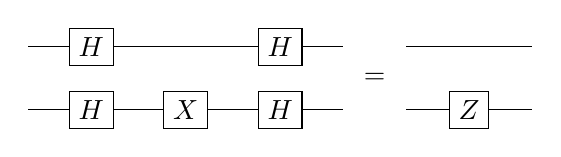
\begin{tikzpicture}
        \node at (0, 0) {$=$};

        \node (2) at (-1.2, 0.4) [rectangle, draw=black] {$H$};
        \node (5) at (-1.2, -0.4) [rectangle, draw=black] {$H$};
        \node (1) at (-3.6, 0.4) [rectangle, draw=black] {$H$};
        \node (3) at (-3.6, -0.4) [rectangle, draw=black] {$H$};
        \node (4) at (-2.4, -0.4) [rectangle, draw=black] {$X$};

        \draw (-4.4, 0.4)--(1);
        \draw (1)--(2);
        \draw (-4.4, -0.4)--(3);
        \draw (2)--(-0.4, 0.4);
        \draw (5)--(-0.4, -0.4);
        \draw (5)--(4);
        \draw (3)--(4);

        \node (z) at (1.2, -0.4) [rectangle, draw=black] {$Z$};
        \draw (z)--(0.4, -0.4);
        \draw (z)--(2, -0.4);
        \draw (0.4, 0.4)--(2, 0.4);
    \end{tikzpicture}
\end{figure}

\begin{figure}[H]
    \centering
    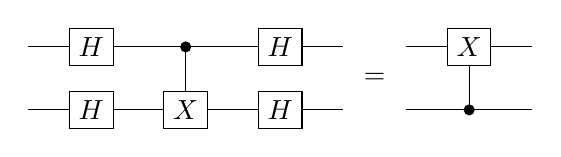
\begin{tikzpicture}
        \node at (0, 0) {$=$};

        \node (2) at (-1.2, 0.4) [rectangle, draw=black] {$H$};
        \node (5) at (-1.2, -0.4) [rectangle, draw=black] {$H$};
        \node (1) at (-3.6, 0.4) [rectangle, draw=black] {$H$};
        \node (3) at (-3.6, -0.4) [rectangle, draw=black] {$H$};
        \node (4) at (-2.4, -0.4) [rectangle, draw=black] {$X$};

        \draw (-4.4, 0.4)--(1);
        \draw (1)--(2);
        \draw (-4.4, -0.4)--(3);
        \draw (2)--(-0.4, 0.4);
        \draw (5)--(-0.4, -0.4);
        \draw (5)--(4);
        \draw (3)--(4);
        \draw (4)--(-2.4, 0.4);
        \fill (-2.4, 0.4) circle (2pt);

        \node (z) at (1.2, 0.4) [rectangle, draw=black] {$X$};

        \fill (1.2, -0.4) circle (2pt);
        \draw (z)--(1.2, -0.4);
        \draw (z)--(0.4, 0.4);
        \draw (z)--(2, 0.4);
        \draw (0.4, -0.4)--(2, -0.4);
    \end{tikzpicture}
\end{figure}

\begin{enumerate}
    \item $f(x)=0$
    \begin{figure}[H]
        \centering
        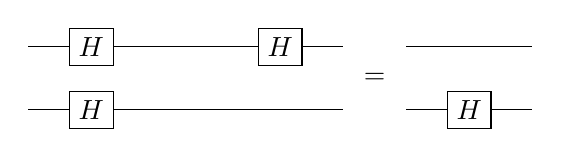
\begin{tikzpicture}
            \node at (0, 0) {$=$};
    
            \node (2) at (-1.2, 0.4) [rectangle, draw=black] {$H$};
            \node (1) at (-3.6, 0.4) [rectangle, draw=black] {$H$};
            \node (3) at (-3.6, -0.4) [rectangle, draw=black] {$H$};
    
            \draw (-4.4, 0.4)--(1);
            \draw (1)--(2);
            \draw (-4.4, -0.4)--(3);
            \draw (2)--(-0.4, 0.4);
            \draw (3)--(-0.4, -0.4);
    
            \node (z) at (1.2, -0.4) [rectangle, draw=black] {$H$};
            \draw (z)--(0.4, -0.4);
            \draw (z)--(2, -0.4);
            \draw (0.4, 0.4)--(2, 0.4);
        \end{tikzpicture}
    \end{figure}
    \item $f(x)=x$
    \begin{figure}[H]
        \centering
        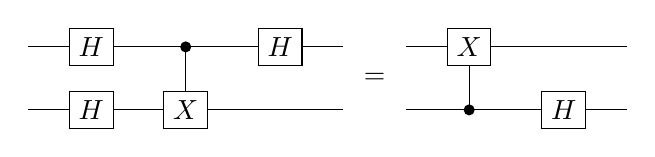
\begin{tikzpicture}
            \node at (0, 0) {$=$};
    
            \node (2) at (-1.2, 0.4) [rectangle, draw=black] {$H$};
            \node (1) at (-3.6, 0.4) [rectangle, draw=black] {$H$};
            \node (3) at (-3.6, -0.4) [rectangle, draw=black] {$H$};
            \node (4) at (-2.4, -0.4) [rectangle, draw=black] {$X$};
    
            \draw (-4.4, 0.4)--(1);
            \draw (1)--(2);
            \draw (-4.4, -0.4)--(3);
            \draw (2)--(-0.4, 0.4);
            \draw (4)--(-0.4, -0.4);
            \draw (3)--(4);
            \draw (4)--(-2.4, 0.4);
            \fill (-2.4, 0.4) circle (2pt);
    
            \node (z) at (1.2, 0.4) [rectangle, draw=black] {$X$};
            \node (H) at (2.4, -0.4) [rectangle, draw=black] {$H$};
    
            \fill (1.2, -0.4) circle (2pt);
            \draw (z)--(1.2, -0.4);
            \draw (z)--(0.4, 0.4);
            \draw (z)--(3.2, 0.4);
            \draw (0.4, -0.4)--(H);
            \draw (H)--(3.2, -0.4);
        \end{tikzpicture}
    \end{figure}
    \item $f(x)=\bar{x}$
    \begin{figure}[H]
        \centering
        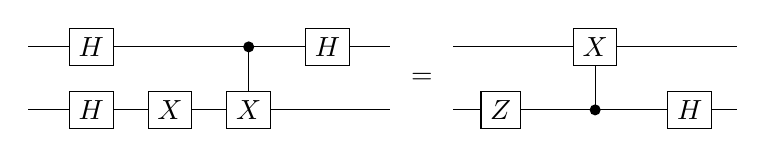
\begin{tikzpicture}
            \node at (0, 0) {$=$};
    
            \node (2) at (-1.2, 0.4) [rectangle, draw=black] {$H$};
            \node (1) at (-4.2, 0.4) [rectangle, draw=black] {$H$};
            \node (3) at (-4.2, -0.4) [rectangle, draw=black] {$H$};
            \node (4) at (-3.2, -0.4) [rectangle, draw=black] {$X$};
            \node (5) at (-2.2, -0.4) [rectangle, draw=black] {$X$};
    
            \draw (-5, 0.4)--(1);
            \draw (1)--(2);
            \draw (-5, -0.4)--(3);
            \draw (2)--(-0.4, 0.4);
            \draw (5)--(-0.4, -0.4);
            \draw (5)--(4);
            \draw (3)--(4);
            \draw (5)--(-2.2, 0.4);
            \fill (-2.2, 0.4) circle (2pt);
            
            \node (z) at (1, -0.4) [rectangle, draw=black] {$Z$};
            \node (x) at (2.2, 0.4) [rectangle, draw=black] {$X$};
            \node (H) at (3.4, -0.4) [rectangle, draw=black] {$H$};
    
            \fill (2.2, -0.4) circle (2pt);
            \draw (x)--(2.2, -0.4);
            \draw (x)--(0.4, 0.4);
            \draw (x)--(4, 0.4);
            \draw (0.4, -0.4)--(z);
            \draw (z)--(H);
            \draw (H)--(4, -0.4);
        \end{tikzpicture}
    \end{figure}
    \item $f(x)=1$
    \begin{figure}[H]
        \centering
        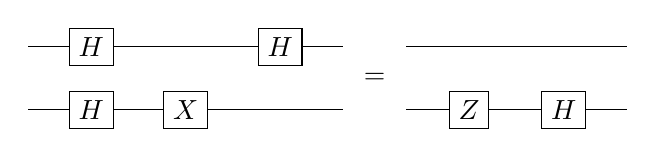
\begin{tikzpicture}
            \node at (0, 0) {$=$};
    
            \node (2) at (-1.2, 0.4) [rectangle, draw=black] {$H$};
            \node (1) at (-3.6, 0.4) [rectangle, draw=black] {$H$};
            \node (3) at (-3.6, -0.4) [rectangle, draw=black] {$H$};
            \node (4) at (-2.4, -0.4) [rectangle, draw=black] {$X$};
    
            \draw (-4.4, 0.4)--(1);
            \draw (1)--(2);
            \draw (-4.4, -0.4)--(3);
            \draw (2)--(-0.4, 0.4);
            \draw (4)--(-0.4, -0.4);
            \draw (3)--(4);
    
            \node (z) at (1.2, -0.4) [rectangle, draw=black] {$Z$};
            \node (H) at (2.4, -0.4) [rectangle, draw=black] {$H$};
    
            \draw (3.2, 0.4)--(0.4, 0.4);
            \draw (0.4, -0.4)--(z);
            \draw (z)--(H);
            \draw (H)--(3.2, -0.4);
        \end{tikzpicture}
    \end{figure}
\end{enumerate}

\subsection{Grover's Trick}
\subsubsection{The Grover Search Algorithm}
The Grover search algorithm performs a search for an entry in an unstructured database, e.g., the title of a book in a library ordered by first author’s name.

The normal setup of the problem assumes that we have been given a subroutine that returns
\begin{align*}
    f(x)=0,\ x\ne a\\
    f(x)=1,\ x=a
\end{align*}
for any $n$-bit integer x , where a is the special value being sought.

In practice, it is told that we are given a black box, which is often called an oracle, containing a quantum circuit (which we do not know in general) that implement the function. The oracle incorporates the usual quantum-computational trick that applies a unitary transformation $U_f$ on an $n$-qubit input and a 1-qubit output as
\begin{align*}
    U_f(\ket{x}_n\ket{y}_1)=\ket{x}_n\ket{y\oplus f(x)}_1
\end{align*}
such that the output isn't flipped or is flipped from 0 to 1 (or vice versa), depending on whether $x=a$ or not. 

We are supposed to start from some quantum state. By repeatedly calling the oracle, we manage to evolve the state toward the unknown $\ket{a}$–so we find it.

If the number of entries in the database is $N$, which can be encoded by $n$ qubits (i.e., $N \lesssim  2^n$).

The Grover algorithm, as we will show, can solve the problem in $\sim \sqrt{N}$ operations. This is an appreciable, though not exponential, speed-up.

\subsubsection{Geometrical Picture}
We use vectors in a two-dimensional plane to illustrate the algorithm. Suppose $\ket{a}$ is the state we want to search. Define $\ket{a_\perp }$ to be the state orthogonal to $\ket{a}$. 

Let us introduce an auxiliary state
\begin{align*}
    \ket{\phi}=\cos\theta\ket{a_\perp}+\sin\theta\ket{a}
\end{align*}
where $\theta$ is the angle bewteen $\ket{\phi}$ and $\ket{a_\perp}$. 

\begin{figure}[H]
    \centering
    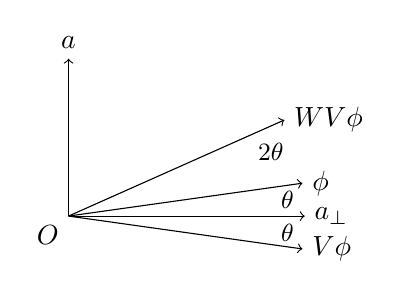
\begin{tikzpicture}
        \draw [->] (0, 0)--(0, 2) node[above] {$\ket{a}$};
        \draw [->] (0, 0)--(3, 0) node[right] {$\ket{a_\perp}$};
        \draw [->] (0, 0)--(8:3) node[right] {$\ket{\phi}$};
        \draw [->] (0, 0)--(-8:3) node[right] {$V\ket{\phi}$};
        \draw [->] (0, 0)--(24:3) node[right] {$WV\ket{\phi}$};
        \node at (0, 0) [below left] {$O$};

        \path (-8:3) -- node[midway,left] {\small$\theta$} (0:3);
        \path (8:3) -- node[midway,left] {\small$\theta$} (0:3);
        \path (8:3) -- node[midway, left] {\small$2\theta$} (24:3);
    \end{tikzpicture}
\end{figure}

We introduce a reflection $V$ with respect to the direction of $\ket{a_\perp}$ as
\begin{align*}
    V=2\ket{a_\perp}\bra{a_\perp}-I=I-2\ket{a}\bra{a}
\end{align*}
The operation flips the sign of the $\ket{a}$ component, while leaving unchanged the components perpendicular to $\ket{a}$. 

We can also introduce a reflection $W$ with respect to the direction of $\ket{\phi}$ as
\begin{align*}
    W=2\ket{\phi}\bra{\phi}-I
\end{align*}

The product of the two reflections is a rotation: $WV$ rotates a vector through the angle $2\theta$ in the direction from $\ket{a_\perp}$ to $\ket{\phi}$. 

Each subsequent application of $WV$ increases the angle bewteen the final state and $\ket{a_\perp}$ by another $2\theta$. A proper choice of the number of $WV$ applications can approach $\ket{a}$ with an error in angle no more than $\theta$. 

\paragraph{How to Relate \texorpdfstring{$V$}. to the Oracle?}
How does the oracle fit into the algorithm that repeatedly rotates a quantum state? The answer is that the reflection of $V$ can be straightforwardly implemented with a call of the black box $U_f$.

\begin{align*}
    V\ket{x}=\left\{\begin{array}{ll}
        \ket{x} & x\ne a\\
        -\ket{a} & x=a
    \end{array}\right.
\end{align*}
This is nothing but $(-1)^{f(x)}\ket{x}$, so we need a trick to make the effect of $U_f$ merely a sign change. 

This is done by initializing the output qubit into the state
\begin{align*}
    H\ket{1}=\frac{1}{\sqrt{2}}(\ket{0}-\ket{1})
\end{align*}
before the application of $U_f$. 

Convince myself that
\begin{align*}
    U_f(\ket{x}\otimes H\ket{1})=(-1)^{f(x)}\ket{x}\otimes H\ket{1}
\end{align*}

Interestingly, the application of $U_f$ on the output qubit can be regarded as the identity, so it is never entangled with the input qubits and remains a constant state throughout the algorithm.

Therefore, for an arbitrary n-qubit input state $\ket{\Psi}=\sum\limits_x \alpha_x\ket{x}$, we have explanied how to implemented
\begin{align*}
    U_f(\ket{\Psi}\otimes H\ket{1})=[\ket{\Psi}-2\ket{a}\braket{a|\Psi}]\otimes H\ket{1}
\end{align*}

\paragraph{How to Choose \texorpdfstring{$\ket{\phi}$}. and Construct \texorpdfstring{$W$}. ?}
Now, the construction of $W$ is closely tied to the choice of the auxiliary state $\ket{\phi}$. We expect the algorithm should work for any $n$-qubit $\ket{a}$. So $\ket{\phi}$ shouldn't be biased toward any $n$-qubit basis vector, We can choose, e.g.,
\begin{align*}
    \ket{\phi}=H^{\otimes n}\ket{0}_n=\frac{1}{2^{n/2}}\sum_{x=0}^{2^n-1}\ket{x}_n
\end{align*}
where $\ket{\phi}$ is easy to prepare, and almost orthogonal to any $\ket{x}_n$. 

As well consider the construction of $-W$
\begin{align*}
    -W=1-2\ket{\phi}\bra{\phi}=H^{\otimes n}(1-2\ket{00\dots0}\bra{00\dots0})H^{\otimes n}
\end{align*}
Notice that $H^{\otimes n}$ is its own inverse. 

Now we need an operation\\ $W'=1-2\ket{00\dots0}\bra{00\dots0}$, which obeys
\begin{align*}
    W' \ket{x}_n=\left\{ \begin{array}{ll}
        \ket{x}_n & x\ne 00\dots0\\
        -\ket{x}_n & x=00\dots0
    \end{array} \right.
\end{align*}

One can verify that 
\begin{align*}
    W' =X^{\otimes n}(C^{n-1} Z)X^{\otimes n}
\end{align*}
where $C^{n-1}Z$ is the $(n-1)$-fold controlled-$Z$ gate. 

\subsubsection{Performance by Geometrical Analysis}
As we discussed in the geometrical picture, each application of $WV$ reduces the angle between the resulting state and $\ket{a}$ by $2\theta$.

With our choice of $\ket{\phi}$,
\begin{align*}
    \cos\left( \frac{\pi}{2}-\theta \right)=\braket{a|\phi}=2^{-n/2}\approx \frac{1}{\sqrt{N}}
\end{align*}

For large $\sqrt{N}$, it's fairly accurate that $\theta\approx 2^{-n/2}$. To rotate $\ket{\phi}$ to $\ket{a}$, we can apply an integral number of $WV$s. A proper choice of the number is as close as possible to
\begin{align*}
    \frac{\frac{\pi}{2}}{2\theta}=\frac{\pi}{4}2^{n/2}\sim \sqrt{N}
\end{align*}
and the error in angle is no more than $\theta \sim 1/\sqrt{N}$. 

If we now measure the input qubits, we have a very high probability to obtain the desired $\ket{a}$. We can repeat the whole procedure a few times to make sure we successfully find $\ket{a}$ in a practical sense.

\subsection{Quantum Supremacy}

%TODO readbook J. D. Hidary, Quantum Computing: An Applied Approach, 2nd Ed. (Springer, 2021), Chap. 8.6